\documentclass{standalone}
\usepackage{pgfplots}
\pgfplotsset{compat=1.18}
\usetikzlibrary{arrows.meta}

\begin{document}
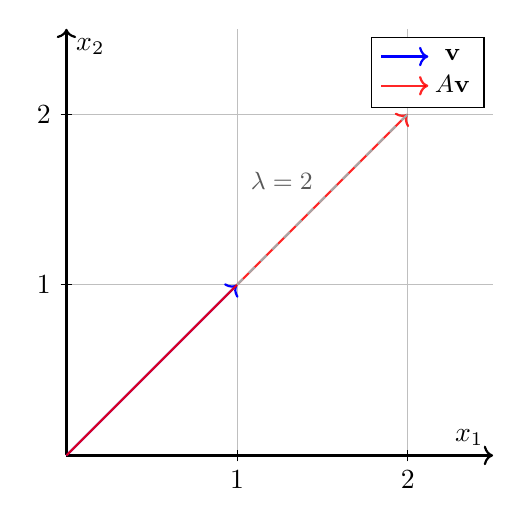
\begin{tikzpicture}
    \begin{axis}[
        axis lines=middle,
        xmin=0, xmax=2.5,
        ymin=0, ymax=2.5,
        xtick={0,1,2},
        ytick={0,1,2},
        xlabel={$x_1$},
        ylabel={$x_2$},
        width=7cm,
        height=7cm,
        axis line style={->,thick},
        tick style={black},
        clip=false,
        grid=both,
        legend style={font=\small},
    ]
        % Original vector
        \addplot[->, thick,blue] coordinates {(0,0) (1,1)};
        \addlegendentry{$\mathbf{v}$}

        % Transformed vector (eigenvector scaled)
        \addplot[->, thick,red,opacity=0.85] coordinates {(0,0) (2,2)};
        \addlegendentry{$A\mathbf{v}$}

        % Dashed line showing scaling
        \addplot[thick, dashed,gray!70] coordinates {(1,1) (2,2)};

        % Labels
        \node[gray!70!black,above left,font=\small] at (axis cs:1.5,1.5) {$\lambda = 2$};
    \end{axis}
\end{tikzpicture}
\end{document}
